\documentclass{article}
\usepackage[utf8]{inputenc}
\usepackage[bmatrix]{amsmath}
\usepackage{graphicx}
\graphicspath{ {./images/} }

\title{Numerical Project #1}
\author{Ross Hart}
\date{March 5, 2020}

\begin{document}

\maketitle

\section{Written Report}
\subsection{Using assigned matrices to analyze the methods}
\subsubsection{Write MATLAB codes for Jacobi, Gauss-Seidel, SOR, Steepest Descent and Conjugate Gradient.
Make sure to document the steps in your code.}
Each of these is included as both a .m and a .sage file (you'll need SageMath and Python 3 to run the .sage files, but they are both opensource so you can find them online)
\subsubsection{Solve each system of equations using Jacobi, Gauss-Seidel, SOR, Steepest Descent and Conjugate Gradient methods and record the number of iterations that each method took to converge with a $10^{−6}$ tolerance. Set the maximum number of iterations to 2000.}
To find/see each of the outputs of the x values ask matlab to return x'method'\#, where 'method' is J,GS,SOR,SD,CG (Jacobi, Gauss-Seidel, SOR, Steepest Descent, Conjugate Gradient, respectively), and \# is either 4 for matrix4.txt or 14 for matrix14.txt. As for the k values, I have made a table here:
\begin{center}
 \begin{tabular}{||c | c | c | c | c | c ||} 
 \hline
 Matrix & Jacobi & Gauss-Seidel & SOR & SD & CG \\ [0.5ex] 
 \hline\hline
 4 & 158 & 18 & 14 & $>$ 2000 & 362 \\ 
 \hline
 14 & 33 & 9 & 8 & 15 & 8 \\ [1ex] 
 \hline
\end{tabular}
\end{center}
\subsubsection{Explanation of results obtained in b).}
For this section, I have elected to copy paste the final lines and the figures of the output of the Section1\_1.m file:
\begin{center}
    \begin{verbatim}
The (2) condition number of matrix 4 is 15243
The spectral radii of matrix 4 are 92.475 for jacobi, 691279530297771264.000 for
Gauss-Seidel, and 13148541403911784759296.000 for SOR.
Matrix 4 is Symmetric
Matrix 4 is not positive definite
Matrix 4 is not tridiagonal
The optimal numerically calculated value(s) of omega is/are 0.58, and because the
spectral radius of the Jacobi T matrix is greater than or equal to 1, the formula
for the optimal omega is imaginary
Conjugate gradient of matrix 4 converges in n iterations

The (2) condition number of matrix 14 is 2
The spectral radii of matrix 14 are 0.614 for jacobi, 0.129 for Gauss-Seidel, and
0.100 for SOR.
Matrix 14 is Symmetric
Matrix 14 is positive definite
Matrix 14 is not tridiagonal
The optimal numerically calculated value(s) of omega is/are 0.91,0.92,0.93,0.94,
0.95,0.96,0.97,0.98, and the formula for the optimal omega yields 1.118
Conjugate gradient of matrix 14 converges in n iterations
Elapsed time is 19.503743 seconds.
    \end{verbatim}
 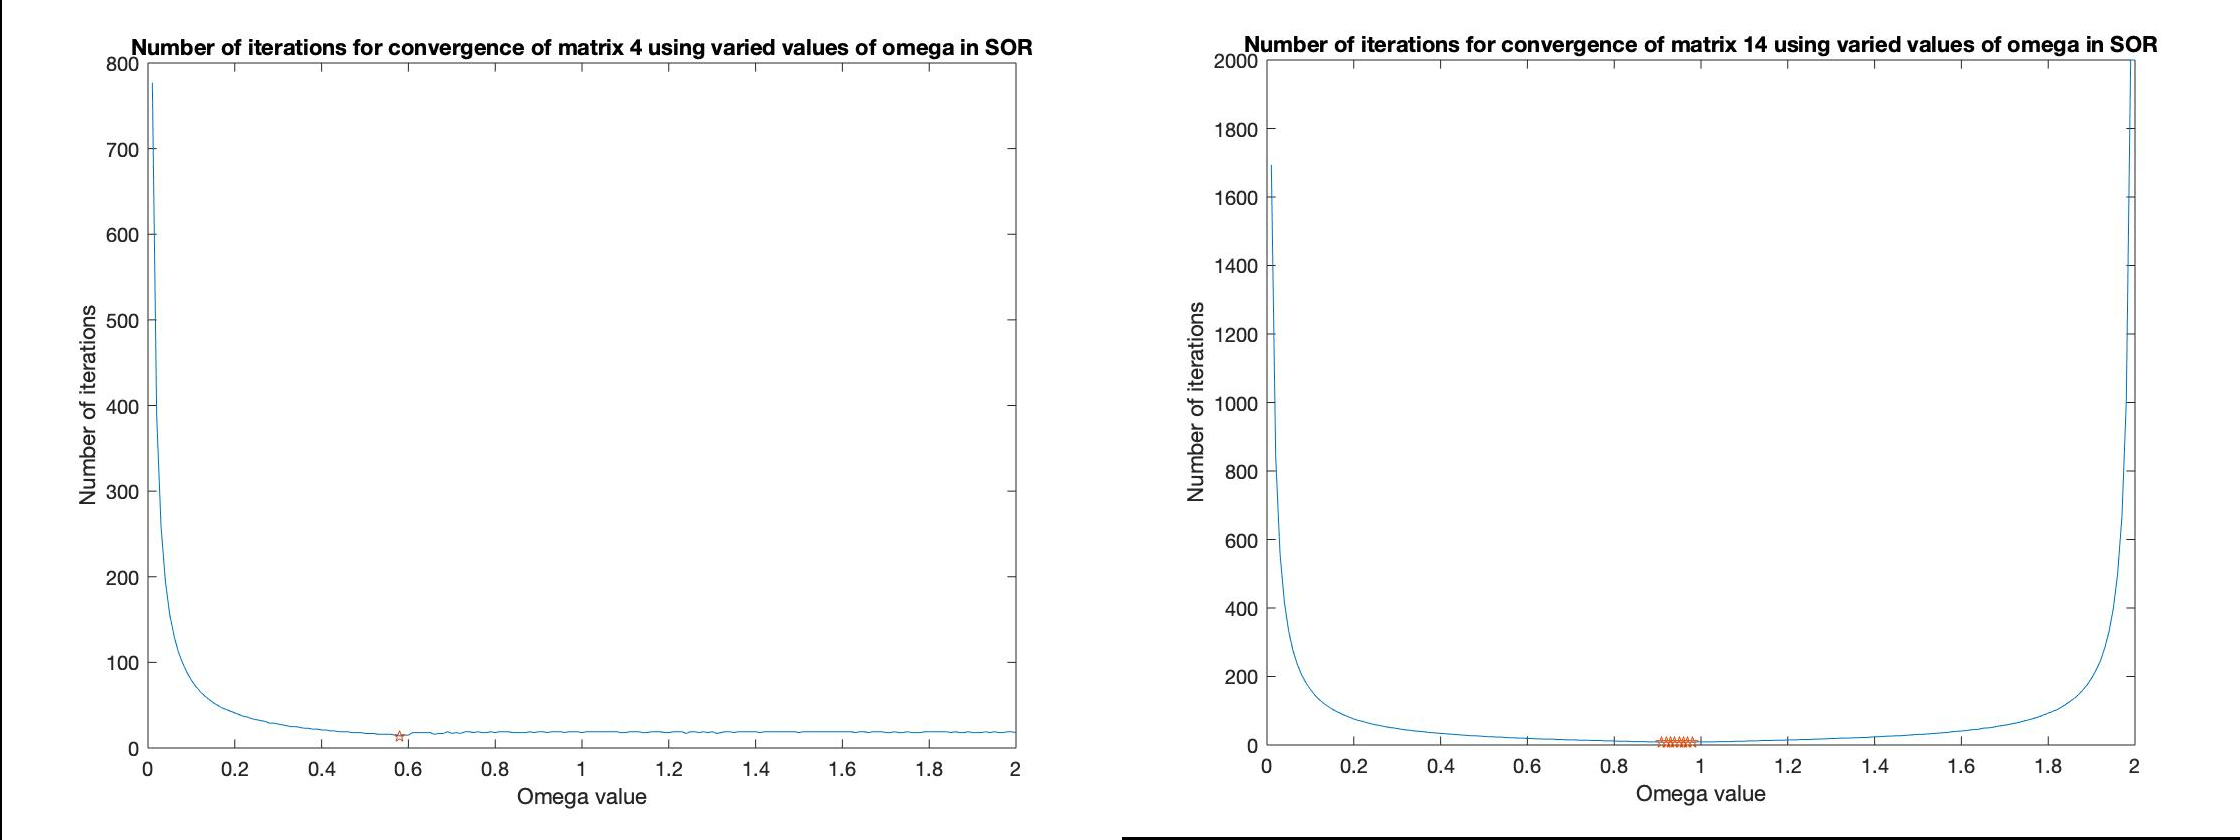
\includegraphics[width=150mm,scale=0.5]{Figure1.png}
\end{center}
\subsection{An application problem}
\subsubsection{Write down the matrix form of $P_i$.}
\begin{document}
\[
P_i = \begin{bmatrix} 
    1 & -1/2 & 0 & 0 & \dots \\
    -1/2 & 1 & -1/2 & 0 & \dots \\
    0 & -1/2 & 1 & -1/2 & \dots \\
    \vdots & \vdots & \vdots & \vdots & \ddots\\
    \end{bmatrix}
\]
\subsubsection{Use the five methods seen in class to solve the system for n = 50, 100, and 200 and record the number of iterations each method takes to converge with a tolerance of $10^{-6}$.}
I will, similarly to the above, create the iteration table and post the output lines and the figures associated below:
\begin{center}
 \begin{tabular}{||c | c | c | c | c | c ||} 
 \hline
 Matrix Size & Jacobi & Gauss-Seidel & SOR & SD & CG \\ [0.5ex] 
 \hline\hline
 50 & $>$ 2000 & 1858 & 103 & $>$ 2000 & $>$ 2000 \\

 \hline
 100 & $>$ 2000 & $>$ 2000 & 184 & $>$ 2000 & $>$ 2000 \\ 
 \hline
  200 & $>$ 2000 & $>$ 2000 & 315 & $>$ 2000 & $>$ 2000 \\ [1ex] 
 \hline
\end{tabular}
\end{center}
\begin{center}
    \begin{verbatim}
The (2) condition number of the matrix of size 50 is 1053
The spectral radii of the matrix of size 50 are 0.998 for jacobi, 0.996 for
Gauss-Seidel, and 0.890 for SOR.
The matrix of size 50 is Symmetric
The matrix of size 50 is Positive definite
The matrix of size 50 is tridiagonal, with diagonal elements greater than zero
but the rest less than zero
The optimal numerically calculated value(s) of omega is/are 1.89,1.90,1.91, and
the formula for the optimal omega yields 1.884
Conjugate gradient of the matrix of size 50 does not converge in n iterations

The (2) condition number of the matrix of size 100 is 4134
The spectral radii of the matrix of size 100 are 1.000 for jacobi, 0.999 for
Gauss-Seidel, and 0.965 for SOR.
The matrix of size 100 is Symmetric
The matrix of size 100 is Positive definite
The matrix of size 100 is tridiagonal, with diagonal elements greater than zero
but the rest less than zero
The optimal numerically calculated value(s) of omega is/are 1.94, and the
formula for the optimal omega yields 1.940
Conjugate gradient of the matrix of size 100 does not converge in n iterations

The (2) condition number of the matrix of size 200 is 16373
The spectral radii of the matrix of size 200 are 1.000 for jacobi, 1.000 for
Gauss-Seidel, and 0.986 for SOR.
The matrix of size 200 is Symmetric
The matrix of size 200 is Positive definite
The matrix of size 200 is tridiagonal, with diagonal elements greater than zero
but the rest less than zero
The optimal numerically calculated value(s) of omega is/are 1.97, and the
formula for the optimal omega yields 1.969
Conjugate gradient of the matrix of size 200 converges in n iterations
Elapsed time is 21.345196 seconds.
    \end{verbatim}
     \hspace*{-1.5cm}
    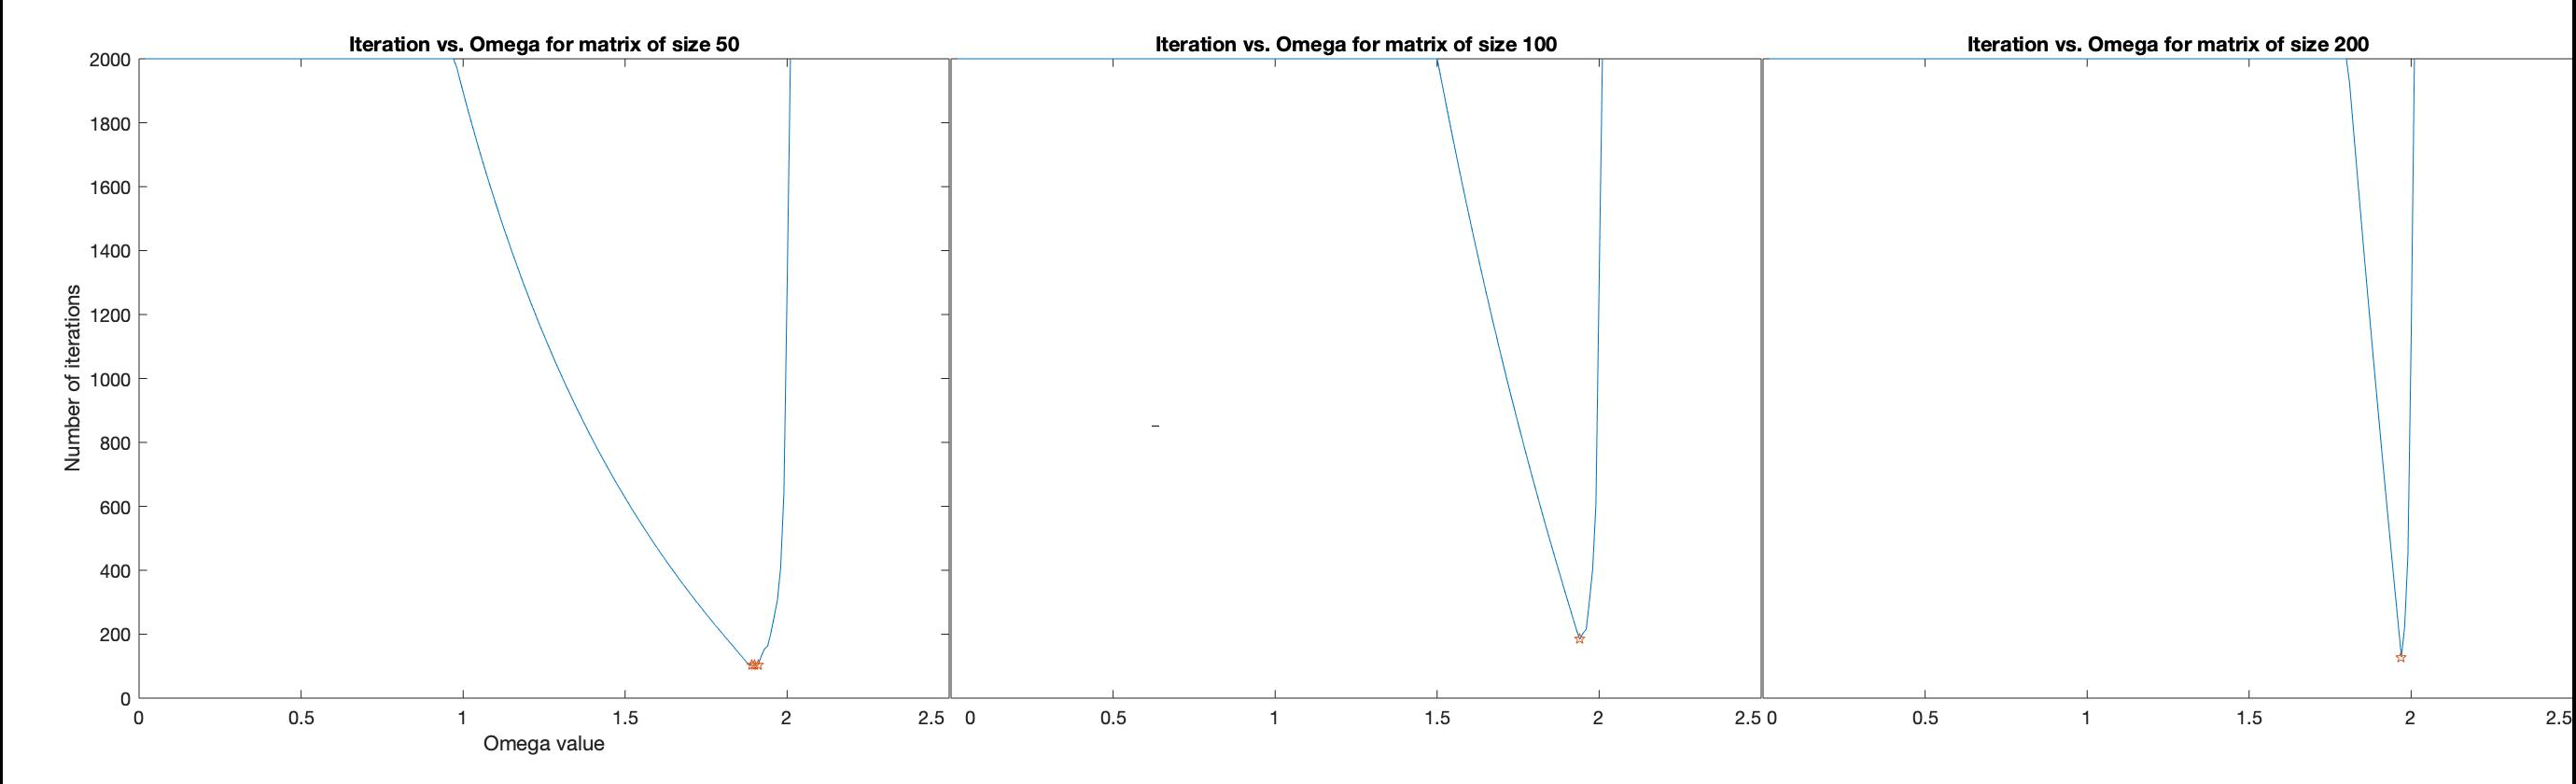
\includegraphics[width=150mm,scale=0.5]{Figure2.png}
\end{center}
\subsubsection{Are the results what you expected? Use the properties of the coefficient matrix, A, etc. to explain your answer.}
These are exactly what we expect. Particularly, the optimal values of omega calculated by the formula align perfectly with those of the numerically generated ones (to about $10^{-3}$), which is precisely our expectation when the tests for positive definite and traditional come back as true.
\subsubsection{Choose a value for α and change the probabilities to α for movement to the right and 1 − α for movement to the left. Repeat parts b) and c). Did anything change? Why or why not?}
I'm gonna say $\alpha=1$, for the free 2 points. That being said, I don't want to repeat the entire thing, so I'm not gonna. 
:)

\end{document}
\end{document}
